\documentclass[12pt,a4paper]{article}
\usepackage[utf8]{inputenc}
\usepackage[spanish]{babel}
\usepackage{amsmath}
\usepackage{amsfonts}
\usepackage{amssymb}
\usepackage{makeidx}
\usepackage{graphicx}
\usepackage[left=2cm,right=2cm,top=2cm,bottom=2cm]{geometry}

\author{Felipe Alvarado Galicia}
\title{SINGULARIDAD DE MANIPULADORES SERIALES}
\date{Profesor:Carlos Enrique Moran Garabito\\
Materia: Cinematica de Robots\\
17 de septiembre de 2019}

\begin{document}
\maketitle
 
\includegraphics[scale=1]{logo1.png}\\
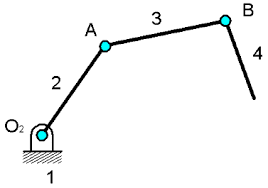
\includegraphics[scale=1]{imag5.png} 
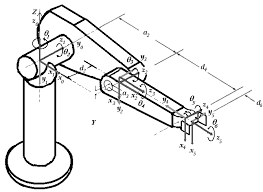
\includegraphics[scale=1]{imag8.png}\\\\\\\\\\\\\\\\\\\\\\\\\\\\\\\\\\\\\\\\\\\\\\

\tableofcontents

\section{Introducción}
Un robot manipulador serie es una cadena cinematica abierta compuesta de una secuencia de elementos estructurales rígidos, denominados eslabones, conectados entre sí a traves de articulaciones, que permiten el movimiento relativo de cada par
de eslabones consecutivos. Al final del ultimo eslabón puedé anadirse una herramienta o dispositivo, denominado elemento terminal.\\

\section{Singularidad de manipuladores seriales redundantes
}
Una singularidad ocurre cuando el órgano terminal de un manipulador serial es incapaz de moverse con una velocidad arbitraria dentro del espacio de trabajo. \\
Esta situación conduce a una solución físicamente irrealizable del análisis de velocidad inverso. Tradicionalmente, el análisis de singularidades, las llamadas “pesadillas cinemáticas” por Hollerbach, se ha estudiado extensamente, igualando a cero el determinante de la matriz Jacobiana. No obstante, debido a que la matriz Jacobiana de un manipulador redundante no es cuadrada, el cálculo de su determinante no tiene sentido. \\
A continuación, algunas contribuciones que abordan el tema de las singularidades en manipuladores seriales. \\
Baker y Wampler II (1988) desarrollaron un procedimiento basado en conceptos de topología matemática para analizar singularidades en manipuladores seriales redundantes que se componen exclusivamente de pares prismáticos o de “revoluta”. El mismo Wampler II (1988) aplicó dichos conceptos en la determinación de las trayectorias factibles que permitan al manipulador abandonar la singularidad en que se encuentra. Ramdane-Cherif et al. (1996) resuelven el análisis de velocidad inverso mediante redes neuronales y de esta manera, analizan la redundancia del manipulador. \\
Sin duda, la teoría de tornillos infinitesimales es una alternativa confiable que permite de una forma sistemática y exacta explicar la naturaleza física de las singularidades. \\
Lipkin y Duffy (1985) mostraron que una singularidad está presente cuando la “cilindroide”, generada entre dos tornillos coaxiales, degenera en una línea. \\
Cuando el determinante de una matriz es cero, condición necesaria para la existencia de la singularidad en manipuladores seriales no redundantes, existe dependencia lineal entre las columnas que la componen. Esta situación permite ubicar como una primera aproximación los posibles elementos que provocan la singularidad. Chevallier (1995) desarrolló un algoritmo basado en el álgebra de Lie para probar la dependencia lineal en conjuntos de tornillos. Podhorodeski et al. (1993) investigó la pérdida de movilidad en manipuladores redundantes agrupando los tornillos asociados a los pares cinemáticos del manipulador linealmente dependientes. \\
Es interesante mencionar que, si bien es cierto, existe una cantidad bastante respetable de contribuciones que tratan el problema de las singularidades en temas como la identificación y la caracterización de singularidades, sorprendentemente, el tema de escape de singularidades ha llamado poco la atención. \\
El primer estudio formal que trata del tema del escape de singularidades se debe a Hunt (1986), quien recurrió a la matriz de cofactores de la matriz Jacobiana y a la teoría de sistemas de tornillos para detectar la singularidad y al tornillo responsable de causarla. Cuando un manipulador serial no redundante pierde un grado de libertad, el rango de la correspondiente matriz Jacobiana es 5, por lo tanto se tienen cinco tornillos linealmente independientes con un tornillo recíproco común. Hunt (1986) determinó que en una configuración singular, el tornillo que es linealmente dependiente, no interviene en la determinación del tornillo que es recíproco. Un resultado similar fue reportado previamente por Sugimoto et al. (1982). \\
Parikian (1996) empleó los determinantes de la matriz Jacobiana y la matriz Gramiana para determinar la proximidad de singularidades en manipuladores seriales no redundantes. La combinación de los gradientes de esas matrices provee información para liberar al manipulador de la singularidad en que se encuentra. En ese mismo año, Karger (1996) utilizó el álgebra de Lie para describir las posibles configuraciones singulares en manipuladores seriales no redundantes. \\
En un trabajo previo Rico et al. (1995) introdujeron un método para identificar a los tornillos que provocan dicha singularidad, dado un manipulador serial no redundante en una configuración singular. A diferencia de los procedimientos anteriormente mencionados, en particular el de Hunt (1986). El método propuesto por Rico et al. (1995) es aplicable a manipuladores no redundantes que pierden más de un grado de libertad, tarea que se considera además de compleja, extremadamente laboriosa.\\
En este trabajo se extiende el método introducido por Rico et al. (1995), aplicable en manipuladores seriales no redundantes a los manipuladores seriales redundantes.\\

\section{Bibliografia:}
file:///C:/Users/acer/Downloads/609-Texto\\
https://upcommons.upc.edu

\end{document}